\documentclass{beamer}
\usepackage{graphicx}    
\usepackage{listings}    
\usepackage{amsmath}

\lstdefinestyle{matlab}{
    language=Matlab,
    basicstyle=\ttfamily\scriptsize,
}

\title{Domača naloga 1}  % Title of the presentation
\author{Sven Filipčič, 23211164}                   % Author name
\date{11.11.2024}                        % Date of the presentation

\begin{document}

% Title slide
\begin{frame}
    \titlepage
\end{frame}

% Table of Contents slide
\begin{frame}
    \frametitle{\textbf{Kazalo}}
    \tableofcontents
\end{frame}

% Slide 1: Introduction
\section{Naloga1-1}
\begin{frame}
    \frametitle{Naloga1-1}
    MATLAB koda za branje datoteke:
    
    Datoteka = fopen('naloga1_1.txt', 'r');  -\textit{odpremo txt datoteko} 
    
    fgetl(Datoteka);  -\textit{Preskočimo prvo vrstico}
    
    fgetl(Datoteka);  -\textit{Preskočimo drugo vrstico}
    
    t = textscan(Datoteka, 'f'); -\textit{preostale številke shranimo v t}
    
    fclose(Datoteka); -\textit{zapremo Datoteko }
    
    t = cell2mat(t); -\textit{pretvorimo cell array v matriko}
    
    disp(t); -\textit{izpiše vrednosti t, da preverimo pravilnost}
    
    
\end{frame}

\section{Predstavitev P(t) grafa}
\begin{frame}
    \frametitle{Predstavitev P(t) grafa}
    Vrednosti P sem prebral iz txt datoteke s pomočjo for loopa, kjer sem vsako vrstico prebral posebaj.Graf predstavlja moč P po času t.
    \begin{figure}[ht] 
    \centering
    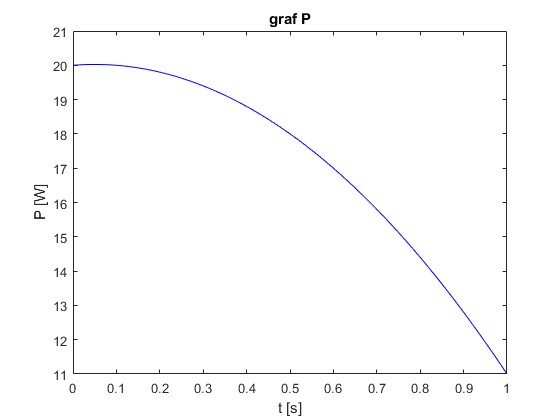
\includegraphics[width=0.8\textwidth]{GrafP.jpg}
    \end{figure}

\end{frame}

% Slide 3: Graph of P(t)
\section{Trapezna formula}
\begin{frame}
    \frametitle{Trapezna formula}
    Formula za izračun integrala z numerično trapezno obliko:
    \[
    \int_a^b f(x) \, dx = \frac{\Delta x}{2} \left( f(x_0) + 2f(x_1) + 2f(x_2) + \dots + 2f(x_{n-1}) + f(x_n) \right)
    \]
    Dobimo rezultat v našem primeru: \textit{17.1665}
    
    Razlika med našim izračunom ter uporabo funkcije trapz je: \textit{-3.5527e-15} kar je praktično nič.
    
\end{frame}

\end{document}